\chapter{Analysis}
\label{ch:analysis}
\graphicspath{{Chapter-Analysis/figures/}}

\section{Data set}

The analyses presented in this thesis use the data from the \ac{LHC} 2013 \pPb at a center-of-mass energy of \pPbenergy with an integrated luminosity of \pPblumi.
The Pb ions had an energy per nucleon of $1.57 \TeV$ and collided with the $4 \TeV$ proton beam resulting in a net longitudinal boost of the center-of-mass system of $\ycm = 0.465$ in the proton direction relative to the ATLAS laboratory frame.
The \pPb\ run was divided into two periods between which the directions of the proton and lead beams were
reversed. 
The data are presented using the convention that the proton beam travels in the forward ($+z$) direction and the lead beam travels in the backward ($-z$) direction.
When the data from these two periods are combined, the \minbias triggers sampled a total luminosity, after prescale, of $24.5~\mu\textrm{b}^{-1}$ and yielded a total of 44 million events over the full centrality.

For results reported as a function of centrality, an additional \ac{HighET} trigger selection is included in the most central bin that requires the total transverse energy in both sides of the \ac{FCal} to be at least 65 \GeV.
The \ac{HighET} trigger sampled a total luminosity of $41.4~\mu\textrm{b}^{-1}$ after prescale and yielded 700 thousand events to the sample.
Events from this trigger are only included in the 0--1\% centrality interval, where the \ac{HighET} trigger is fully efficient.

The azimuthally-dependent results use central events with offline charged-particle multiplicity \Nch of at least 150, where only tracks with $\pt > 400~\MeV$ are counted in this number.
Several \acp{HMT} are included to boost the sample, with offline \Nch cutoffs at 100, 130, 150, 180, 200, and 225 tracks.
These \acp{HMT} provide a crucial 6.7 million events, as the \minbias triggers provide only 200 000 events at $\Nch > 150$.

All events are required to pass a set of \minbias selection criteria.
Events are required to be included in the latest Good Runs List from ATLAS, which rejects events recorded in conjunction with a technical difficulty in the detector.
The \minbias trigger requires either one hit in both sides of the \ac{MBTS} or two hits in one side.
Additional \ac{HighET} and high multiplicity triggers are included in some analysis bins as discussed above.
%% Events with an offline multiplicity lower than the nominal trigger threshold are excluded, as each of these HMTs reaches an efficiency near 1 near their nominal turn-on. This rejects events that fire a trigger in its turn-on region, as these samples can in principle be biased.
%% In practice no significant difference in the results is observed whether or not events in the HMT triggers' turn-ons are included, so using the nominal turn-on multiplicity is sufficient.
A timing cut is placed on the \ac{MBTS} hits in each side such that $|\Delta t_{AC}| < 10~\textrm{ns}$.
No more than one reconstructed \ac{PV} or strong vertex (where a strong vertex has more than 10 tracks or a total \pt of tracks greater than $6~\GeV$) is permitted in each event.
Diffractive events are identified for rejection by a gap of two units of pseudorapidity in event activity on the Pb-going side of the calorimeters \cite{HION-2012-15}.
Pileup events are also discarded using a run-dependent upper limit on the Pb-going \ac{ZDC}.
In addition, events are discarded if an error flag is recorded in the \ac{LAr} or tile calorimeter systems, or if there is an indication that the event was not completely recorded.

\section{Centrality determination}

\begin{figure}[t]
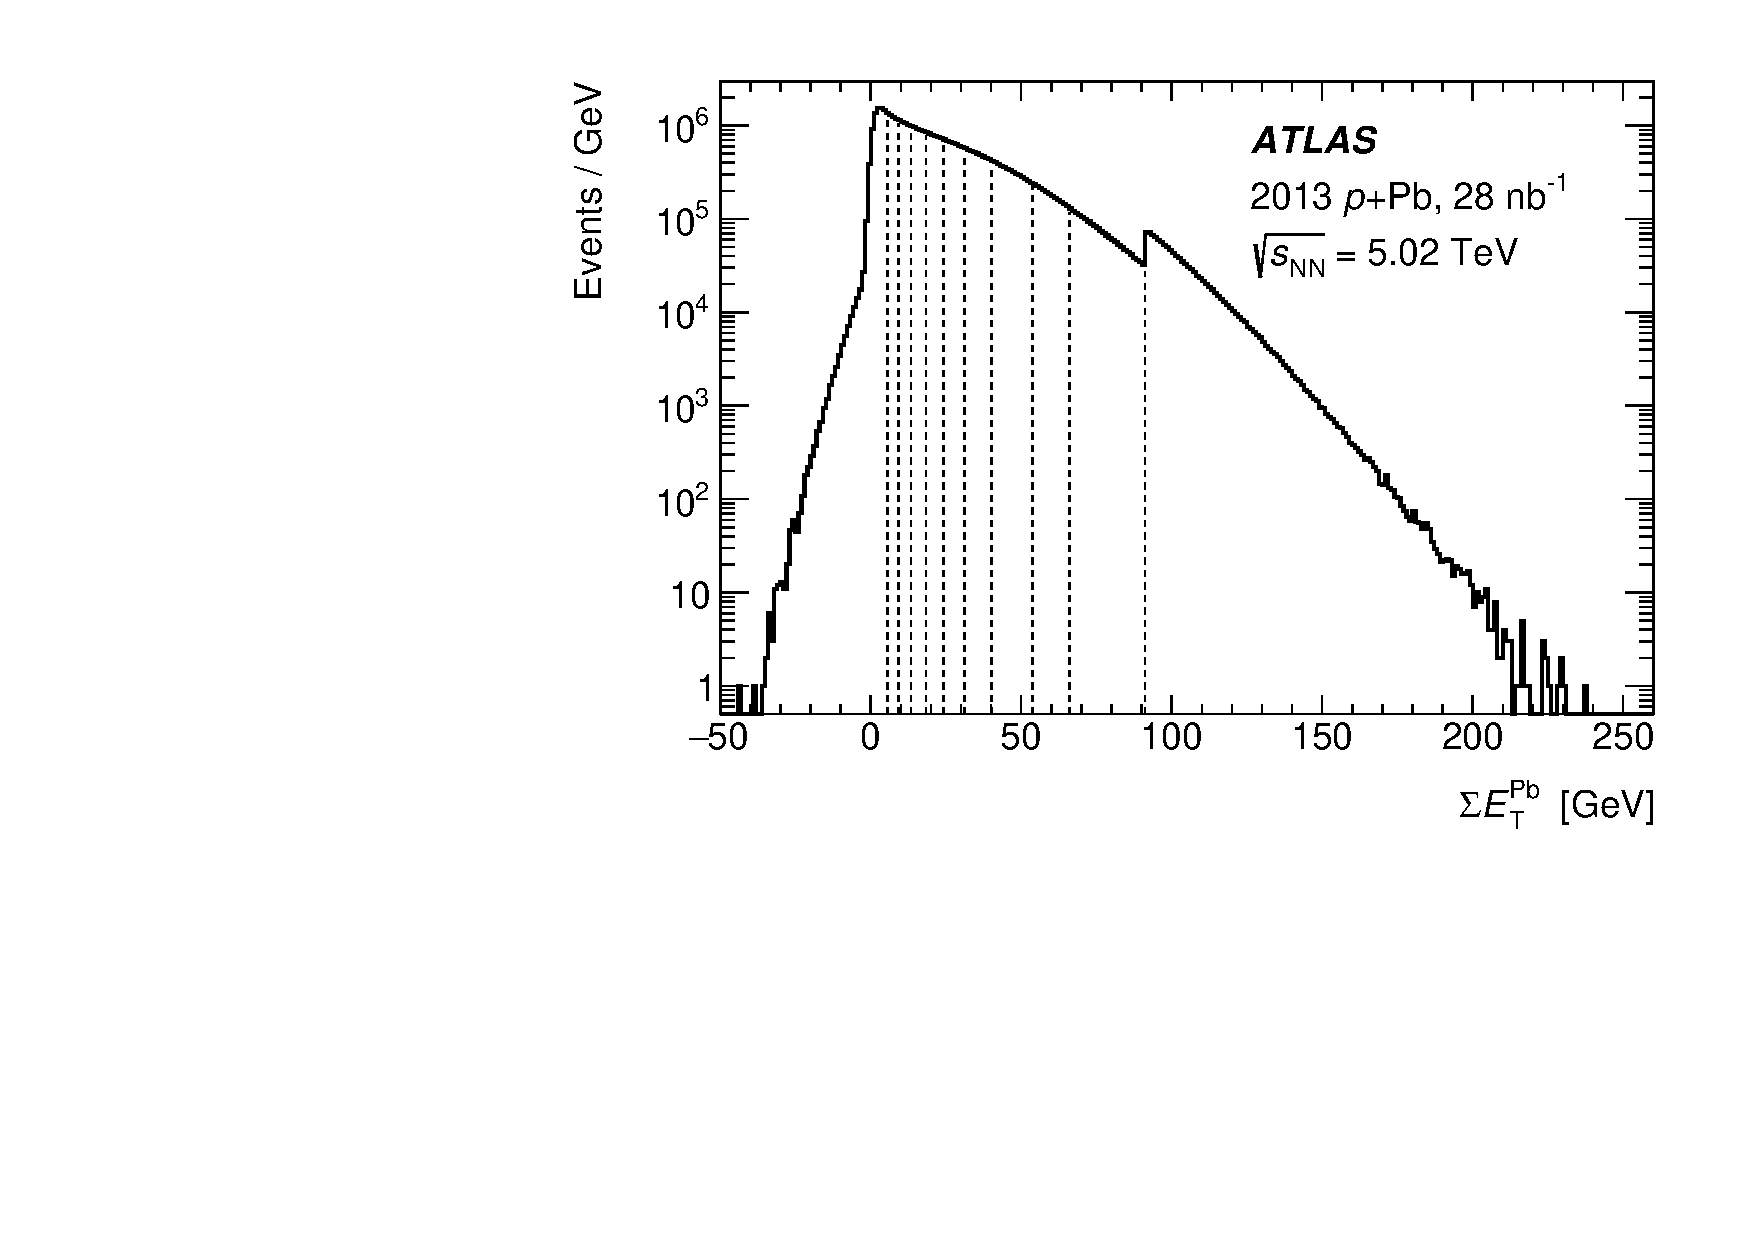
\includegraphics{fcal_et_total.pdf}
\caption{The distribution of the total transverse energy in the \ac{FCal} in the Pb-going direction (\sumETPb) for the events used in the centrality-dependent analysis. Dashed lines are shown at the boundaries of the centrality intervals, and the discontinuity at $\sumETPb = 91.08~\GeV$ corresponds to the lower \sumETPb boundary of the 0--1\% centrality interval.}
\label{fig:fcal_et}
\end{figure}

The centralities of the \pPb\ events are characterized following the procedures described in \Ref{\cite{HION-2012-15}}, using the total transverse energy in the Pb-going side of the \ac{FCal}, \sumETPb.
The use of the \ac{FCal} for measuring centrality has the advantage that it is not sensitive to multiplicity flvuctuations in the kinematic region covered by the inner detector, where the measurements are performed.
Measurements are presented in this paper for the centrality intervals listed in \Cref{table:npart}.
The events selected using the \ac{HighET} trigger are used only in the 0--1\% centrality interval.
\Cref{fig:fcal_et} shows the distribution of \sumETPb\ values obtained from events included in this
measurement.
The discontinuity in the spectrum occurs at the low edge of the 0--1\% centrality interval, above which the \ac{HighET} events are included.

For each centrality interval, the average multiplicity of charged particles with $\pt > 100~\MeV$ and $|\eta| < 1.5$, \avgdNdeta, and the corresponding average number of participating nucleons, \avgNpart, are obtained from a previous publication \cite{HION-2012-15}.
Since this analysis uses finer centrality intervals (no wider than 10\% of the total centrality range) than
those used in \Ref{\cite{HION-2012-15}}, a linear interpolation over the Glauber \avgNpart is used to construct additional values for \avgdNdeta based on the published results.
This interpolation is justified by the result in \Ref{\cite{HION-2012-15}} that charged-particle multiplicity is proportional to \avgNpart in the peripheral region.
The values and uncertainties from this procedure are listed in \Cref{table:npart}.


\renewcommand{\arraystretch}{1.1}
\begin{table}
\begin{center}
\begin{tabular}{r || c | c | c || c}
\hline
 & \multicolumn{3}{c||}{\avgNpart} & \\ \cline{2-4}
Centrality & Glauber & GGCF $\omega_{\sigma} = 0.11$ & GGCF $\omega_{\sigma} = 0.2$ & $\avgdNdeta$\\
\hline \hline
0--1\% & $ 18.2^{+2.6}_{-1.0} $ & $ 24.2^{+1.5}_{-2.1} $ & $ 27.4^{+1.6}_{-4.5} $ & $58.1\ \pm 0.1\ \ \pm 1.9\ $ \\[2pt]
\hline
1--5\% & $ 16.10^{+1.66}_{-0.91} $ & $ 19.5^{+1.2}_{-1.3} $ & $ 21.4^{+1.5}_{-2.0} $ & $45.8\ \pm 0.1\ \ \pm 1.3\ $ \\[2pt]
\hline
5--10\% & $ 14.61^{+1.21}_{-0.82} $ & $ 16.5^{+1.0}_{-1.0} $ & $ 17.5^{+1.1}_{-1.1} $ & $38.5\ \pm 0.1\ \ \pm 1.1\ $ \\[2pt]
\hline
10--20\% & $ 13.05^{+0.82}_{-0.73} $ & $ 13.77^{+0.79}_{-0.81} $ & $ 14.11^{+0.86}_{-0.79} $ & $32.34 \pm 0.05 \pm 0.97$ \\[2pt]
\hline
20--30\% & $ 11.37^{+0.65}_{-0.63} $ & $ 11.23^{+0.62}_{-0.67} $ & $ 11.17^{+0.68}_{-0.62} $ & $26.74 \pm 0.04 \pm 0.80$ \\[2pt]
\hline
30--40\% & $ 9.81^{+0.56}_{-0.57} $ & $ 9.22^{+0.50}_{-0.54} $ & $ 8.97^{+0.60}_{-0.49} $ & $22.48 \pm 0.03 \pm 0.75$ \\[2pt]
\hline
40--50\% & $ 8.23^{+0.48}_{-0.55} $ & $ 7.46^{+0.41}_{-0.43} $ & $ 7.15^{+0.54}_{-0.39} $ & $18.79 \pm 0.02 \pm 0.69$ \\[2pt]
\hline
50--60\% & $ 6.64^{+0.41}_{-0.52} $ & $ 5.90^{+0.36}_{-0.34} $ & $ 5.60^{+0.47}_{-0.30} $ & $15.02 \pm 0.02 \pm 0.62$ \\[2pt]
\hline
60--70\% & $ 5.14^{+0.35}_{-0.43} $ & $ 4.56^{+0.32}_{-0.26} $ & $ 4.32^{+0.41}_{-0.23} $ & $11.45 \pm 0.01 \pm 0.56$ \\[2pt]
\hline
70--80\% & $ 3.90^{+0.24}_{-0.30} $ & $ 3.50^{+0.22}_{-0.18} $ & $ 3.34^{+0.29}_{-0.16} $ & $ \ \  8.49 \pm 0.02 \pm 0.51$ \\[2pt]
\hline
\end{tabular}
\caption{The average number of nucleon participants \avgNpart \cite{HION-2012-15} for each centrality interval in the Glauber model as well as the two choices for the Glauber-Gribov model with color fluctuations (GGCF) \cite{Alvioli:2013vk} (and references therein), along with the average multiplicity with $\pt > 100~\MeV$ and $|\eta| < 1.5$ also obtained from Ref.~\cite{HION-2012-15}. The parameter $\omega_{\sigma}$ represents the size of fluctuations in the nucleon-nucleon cross section. Asymmetric systematic uncertainties are shown for \avgNpart. The uncertainties in \avgdNdeta are given in the order of statistical followed by systematic.}
\label{table:npart}
\end{center}
\end{table}

 

\section{Flow vector determination}

The 2nd-order azimuthal Fourier components $Q_2$ of the energy flow are defined by
\begin{equation}
  Q_2 = \sum_{i}  \et{}_i \begin{pmatrix} \cos 2\phi_i \\ \sin 2\phi_i \end{pmatrix} \; ,\\
\end{equation}
where the sum is taken over calorimeter cells and $\phi_i$ is the ATLAS detector coordinate $\phi$ of the $i$th calorimeter cell.
The two-component elliptic flow vector \qt is defined in terms of $Q_2$, normalized by the 0th-order Fourier component
\begin{equation}
  \qt = \frac{Q_2}{\sum_i \et{}_i } \; .\\
\end{equation}

The elliptic flow used in this analysis is taken from calorimeter cells on the Pb-going side of the detector with $\eta < -2.5$ for period B or $\eta > 2.5$ for period A, which has the beam orientation reversed. This forward cut is made so as to not overlap with the inner detector.

The second-order event plane angle \psit is defined as
\begin{equation}
2\psit = \mathrm{atan2}(\qt{}_{,y},\qt{}_{,x})
\end{equation}
and the magnitude of the flow vector is $|\qt| = \sqrt{\qtx^2 + \qty^2}$.
An equivalent expression of these equations is
\[
\qt = |\qt| e^{i2\psit} = \frac{\sum_i \et{}_i e^{i2\phi_i}}{\sum_i \et{}_i} \; .
\]
A sketch of the relationship of event plane angle to transverse momentum is shown in \Fig{\ref{fig:ep_cartoon}}.

\begin{figure}[t]
  \centering
  \includegraphics[width=\linewidth]{event_plane_cartoon.png}
  \caption{The event plane angle $\psit$ in relation to the elliptic moment of transverse energy. An exaggerated example of the transverse profile in a hydrodynamic system is shown in blue. The pressure gradients are larger along the axis of narrower extent, leading to greater final momentum in that direction.}
\label{fig:ep_cartoon}
\end{figure}

\subsection{First-order correction}
Due to non-uniformities in the calorimeter response in azimuth, the measurement of the \qt vector may be biased. This leads to a non-uniform distribution of event plane angle \psit with an additive term proportional to $\cos (2(\psit - \phi_0))$ which is obviously not physical.
This bias is corrected by subtracting off the mean \qt on a run-by-run basis.
The mean components of the \qt vector are shown in \Fig{\ref{fig:mean_q2}}.
The correction factors are statistically consistent in different multiplicity intervals, so all multiplicities are combined to increase their statistical significance.

\begin{figure}[t]
\centering
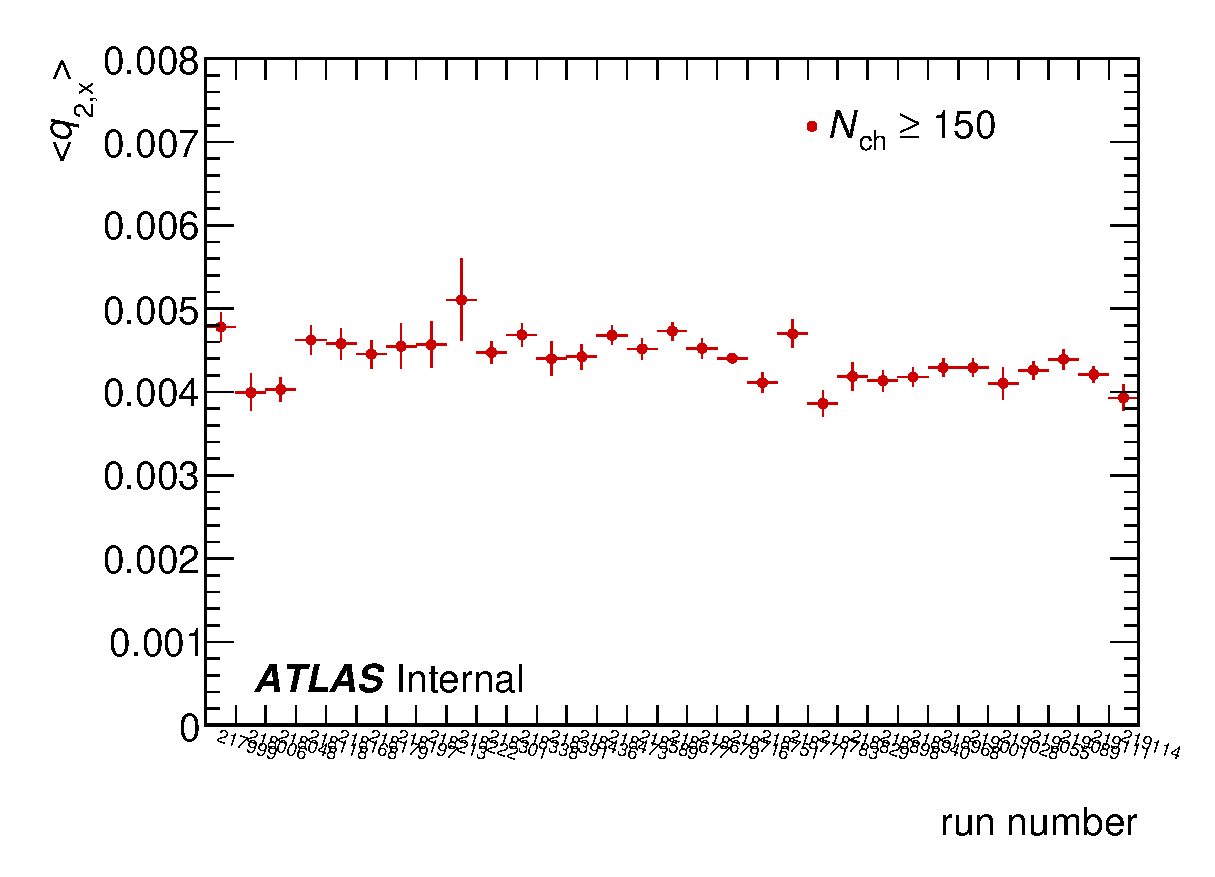
\includegraphics[width=.49\linewidth]{can_qx.eps}
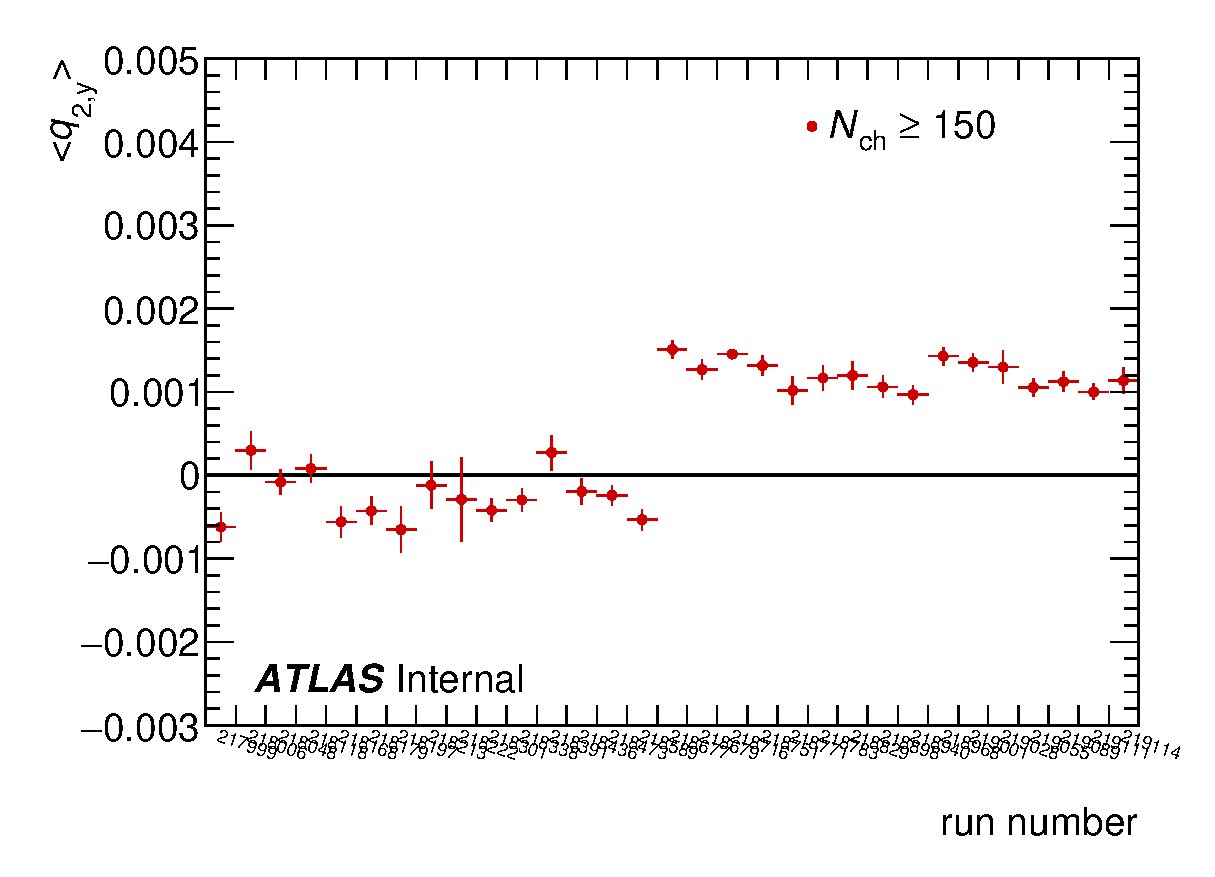
\includegraphics[width=.49\linewidth]{can_qy.eps}
\caption{The average components of the \qt vector $\langle\qtx\rangle$ (left) and $\langle\qty\rangle$ (right) for each run. Runs up to 218589 are from period A, and use $\eta > 2.5$, while runs after this are from period B and use $\eta < -2.5$.}
\label{fig:mean_q2}
\end{figure}

\subsection{Second-order correction}

Some additional non-uniformities persist in the \psit distribution even after correcting for the nonvanishing $\langle\qt\rangle$.
These show up in higher-order Fourier terms like $\cos (4\psit)$ and $\sin(4\psit)$ in the distribution of the event plane angle \psit.
They arise because detector irregularities can lead to higher-order distortions in the distribution of the matrix of products $\qt{}_i \qt{}_j$.
In order to correct for these and make $\langle \qt{}_i \qt{}_j \rangle$ proportional to the identity matrix, the mean-corrected \qt vector is multiplied by the normalized inverse square root of the covariance matrix
\begin{equation}
\frac{1}{\sqrt{N}} \left( \begin{array}{ccc}
  \langle \qty^2 \rangle + D & -\langle\qtx\qty\rangle \\
  -\langle\qtx\qty\rangle & \langle \qtx^2 \rangle + D
  \end{array} \right) \; ,
\end{equation}
where $D = \sqrt{\langle \qtx^2 \rangle \langle \qty^2 \rangle - \langle \qtx \qty \rangle ^2}$ and $N = D\left(\langle \qtx^2 \rangle + \langle\qty^2\rangle + 2D\right)$. The components of the covariance matrix are shown in \Fig{\ref{fig:mean_q2_cov}}. This multiplication causes the corrected \qt vector to have no skew and have the same width in the \qtx and \qty axes.

\begin{figure}[t]
\centering
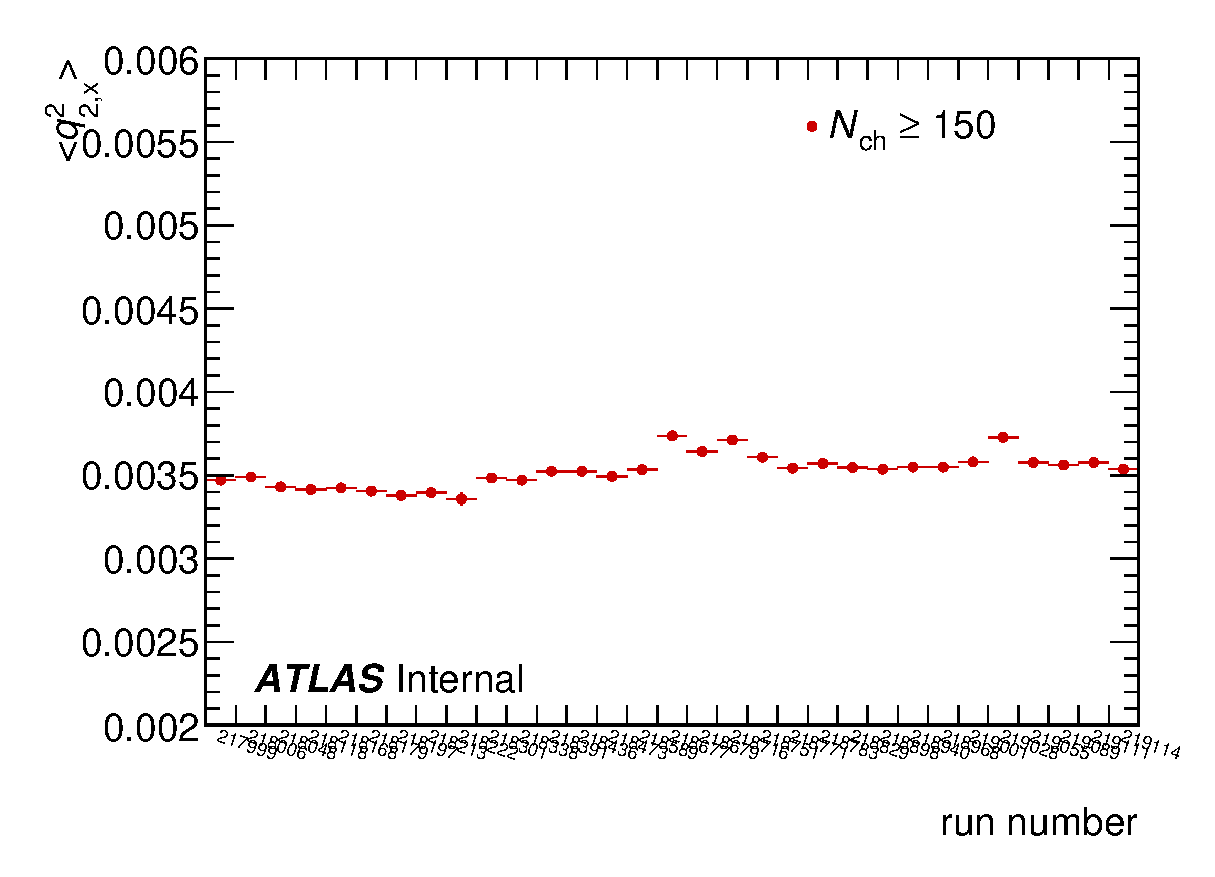
\includegraphics[width=.49\linewidth]{can_qxx.eps}
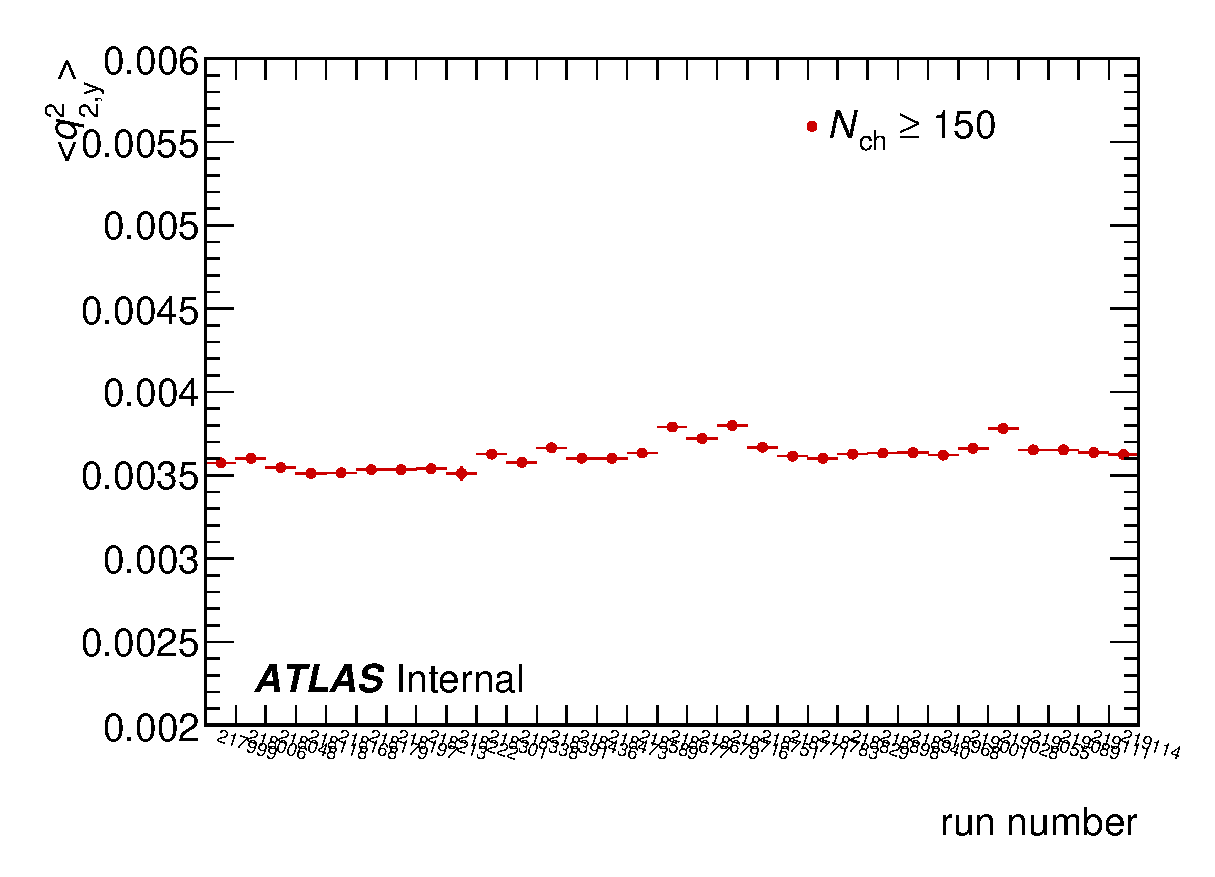
\includegraphics[width=.49\linewidth]{can_qyy.eps}\\
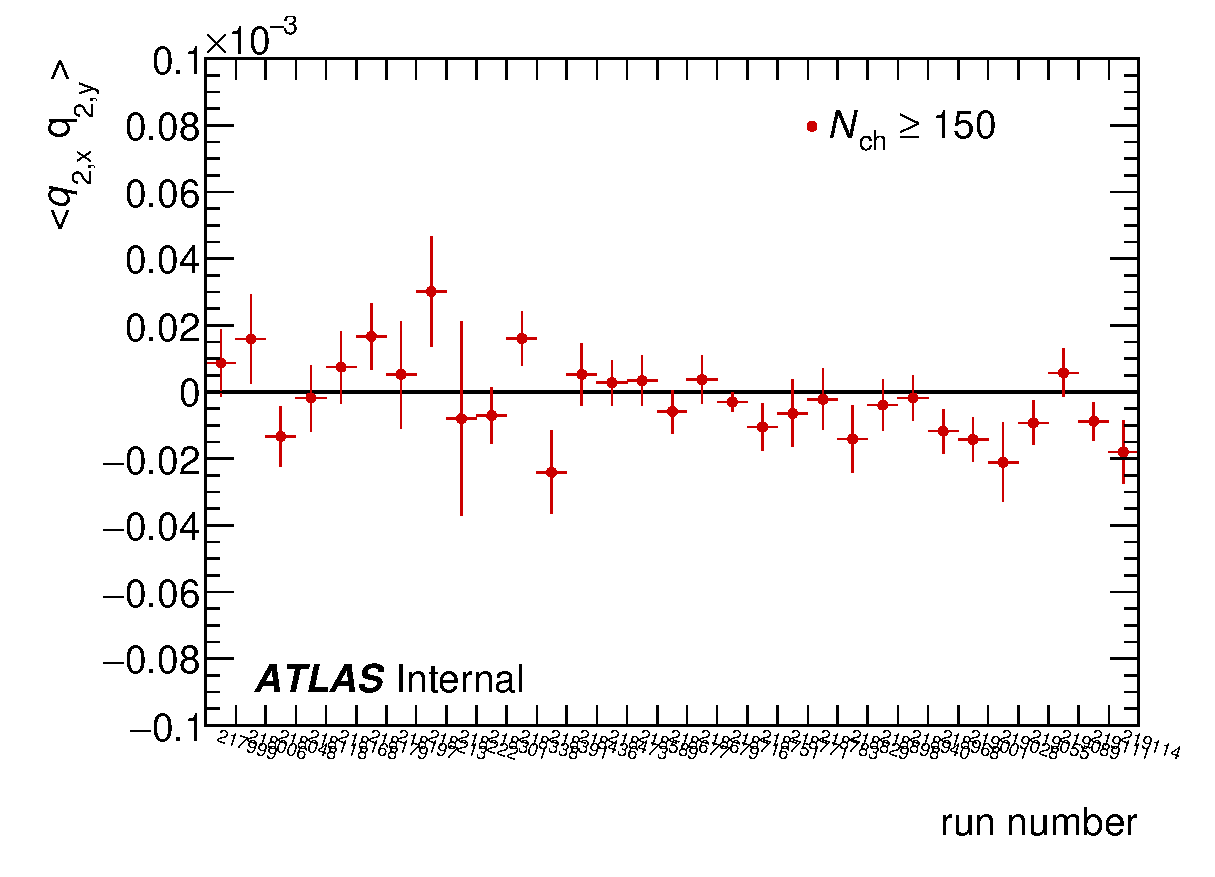
\includegraphics[width=.49\linewidth]{can_qxy.eps}
\caption{The average components of the $<\qt{}_i \qt{}_j>$ matrix for each run. Runs up to 218589 are from period A, and use $\eta > 2.5$, while runs after this are from period B and use $\eta < -2.5$.}
\label{fig:mean_q2_cov}
\end{figure}

As is the case for the mean subtraction correction, the correction factors are consistent over multiplicity so the events are combined for improved statistical significance in the correction.
Once these two corrections are applied run-by-run, the \psit distribution is flat (\Figs{\ref{fig:dNdpsi2_corr}}{\ref{fig:dNdpsi2_corr_binned}}).

\begin{figure}[t]
\centering
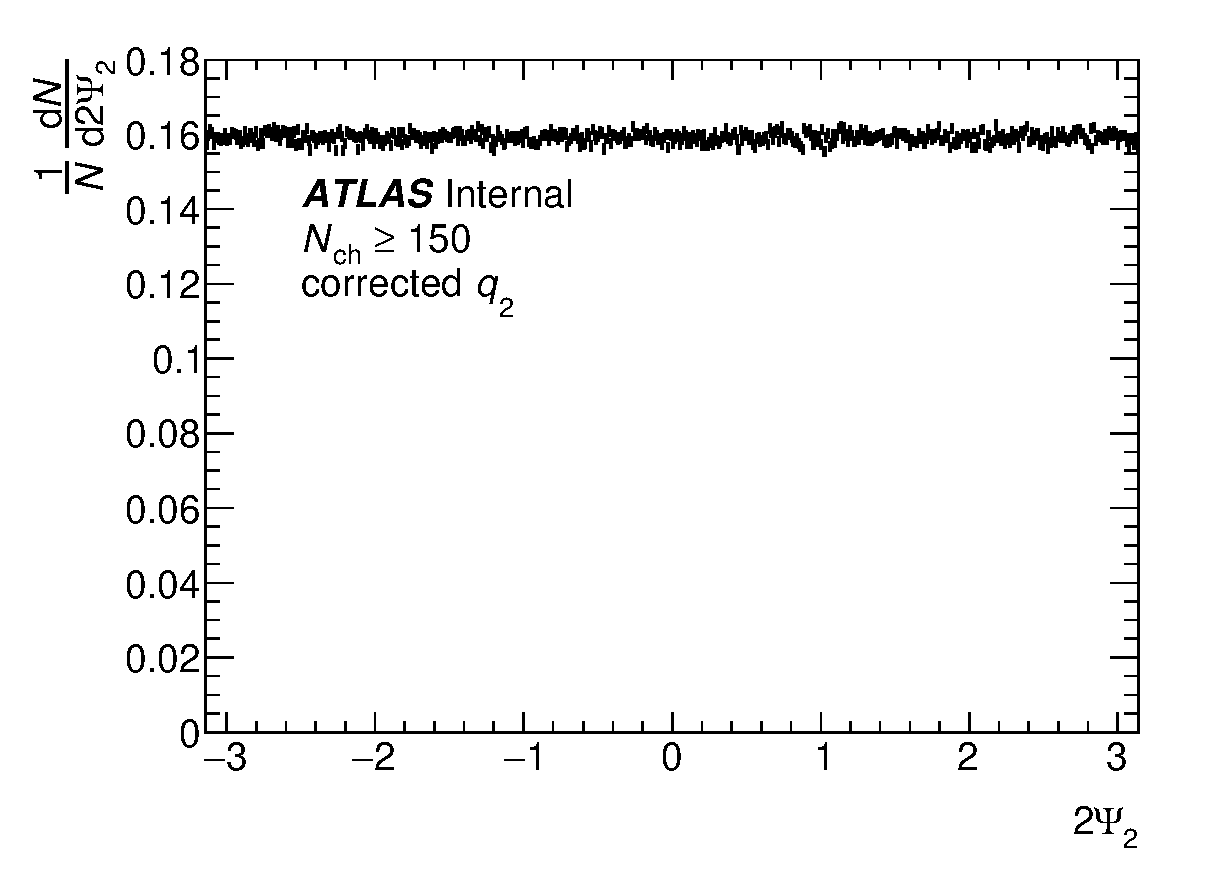
\includegraphics{dNdpsi2.eps}\\
\caption{The distribution of second-order event plane angle after first- and second-order flow vector corrections.}
\label{fig:dNdpsi2_corr}
\end{figure}

\begin{figure}[t]
\centering
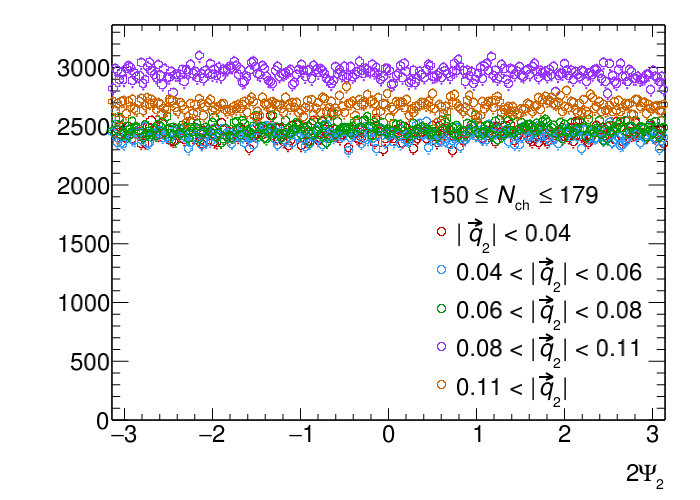
\includegraphics[width=.49\linewidth]{can_psi2_Nch150to179.png}
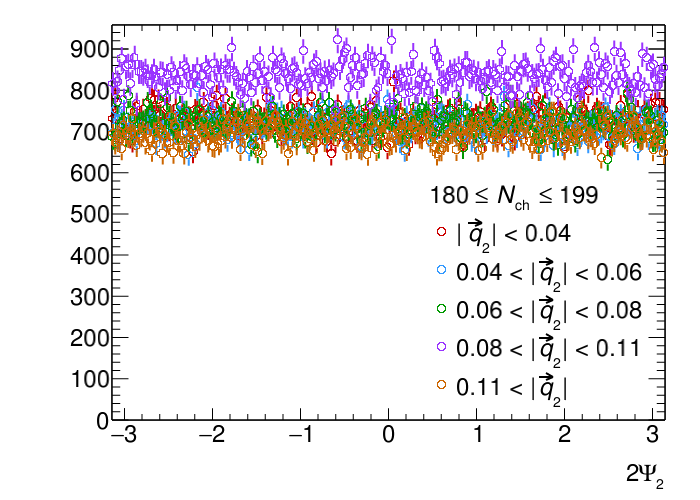
\includegraphics[width=.49\linewidth]{can_psi2_Nch180to199.png}
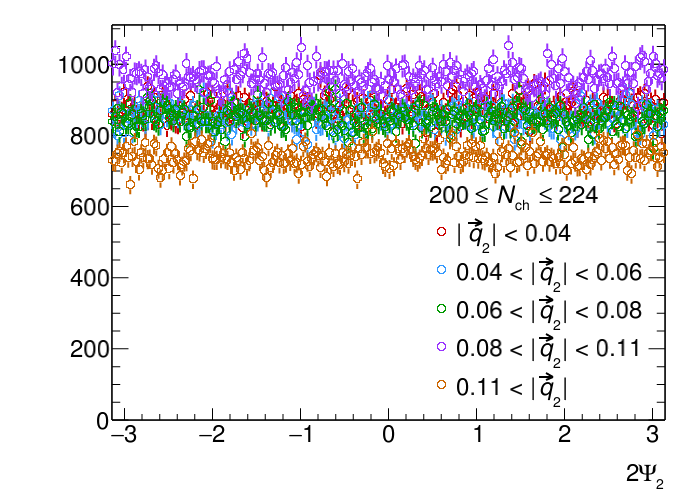
\includegraphics[width=.49\linewidth]{can_psi2_Nch200to224.png}
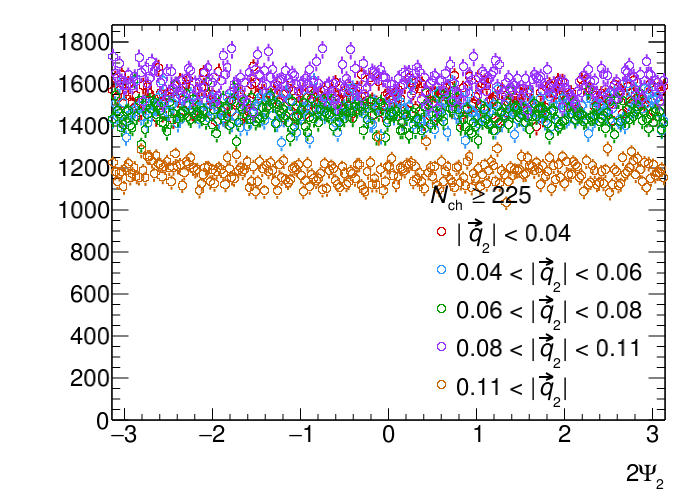
\includegraphics[width=.49\linewidth]{can_psi2_Nch225.png}
\caption{The distribution of second-order event plane angle, in bins of flow vector magnitude $|\qt|$. Each panel shows a different interval of reconstructed charged particle multiplicity \Nch.}
\label{fig:dNdpsi2_corr_binned}
\end{figure}


\subsection{Event plane angular resolution}
\label{subsubsec:epres}

The event plane angular resolution, defined as $\langle \cos(2 \delta \psit) \rangle$ where $\delta \psit$ is the difference between true and measured \psit, is shown in \Fig{\ref{fig:ep_res}} for the calorimeters at $\eta < -2.5$.
The resolution is shown separately for periods A and B, but since they are comparable only the combined resolution is used.
This quantity can be calculated from data using the three-sub-detector method, where two other subdetectors are chosen with rapidity ranges $-2 < \eta< -0.5$ and $0 < \eta < 1.5$.
Here explicit pseudorapidity ranges define each subdetector, with a pseudorapidity gap of 0.5 left in between each subdetector so that biases are not introduced from jets overlapping two subdetectors.
The event plane resolution of the nominal subdetector can be calculated with the following expression.

\begin{equation}
\langle \cos(2 \delta \psit) \rangle = \sqrt{ \frac{\langle \cos(2\psit^A - 2\psit) \rangle \langle \cos(2\psit^B - 2\psit) \rangle }{\langle \cos(2\psit^A - 2\psit^B) \rangle} }\\
\end{equation}
Here $\psit^A$ refers to the event plane measured using calorimeters with $-2 < \eta< -0.5$ and $\psit^B$ refers to that with $0 < \eta < 1.5$.
Each of these additional subdetectors has first- and second-order corrections applied, which are derived for each subdetector in the same way that the corrections are derived for the nominal subdetector with $\eta < -2.5$.
Systematic uncertainties in the event plane resolution are taken from two sources.
The alternate subdetectors are shifted by $\Delta\eta = +0.5$, and the difference in the EP resolution is symmetrized.
Also, the alternate subdetectors are calculated using the \qt from tracks, weighted by their \pt. This difference is also symmetrized, and these two contributions are added in quadrature.

\begin{figure}[t]
\centering
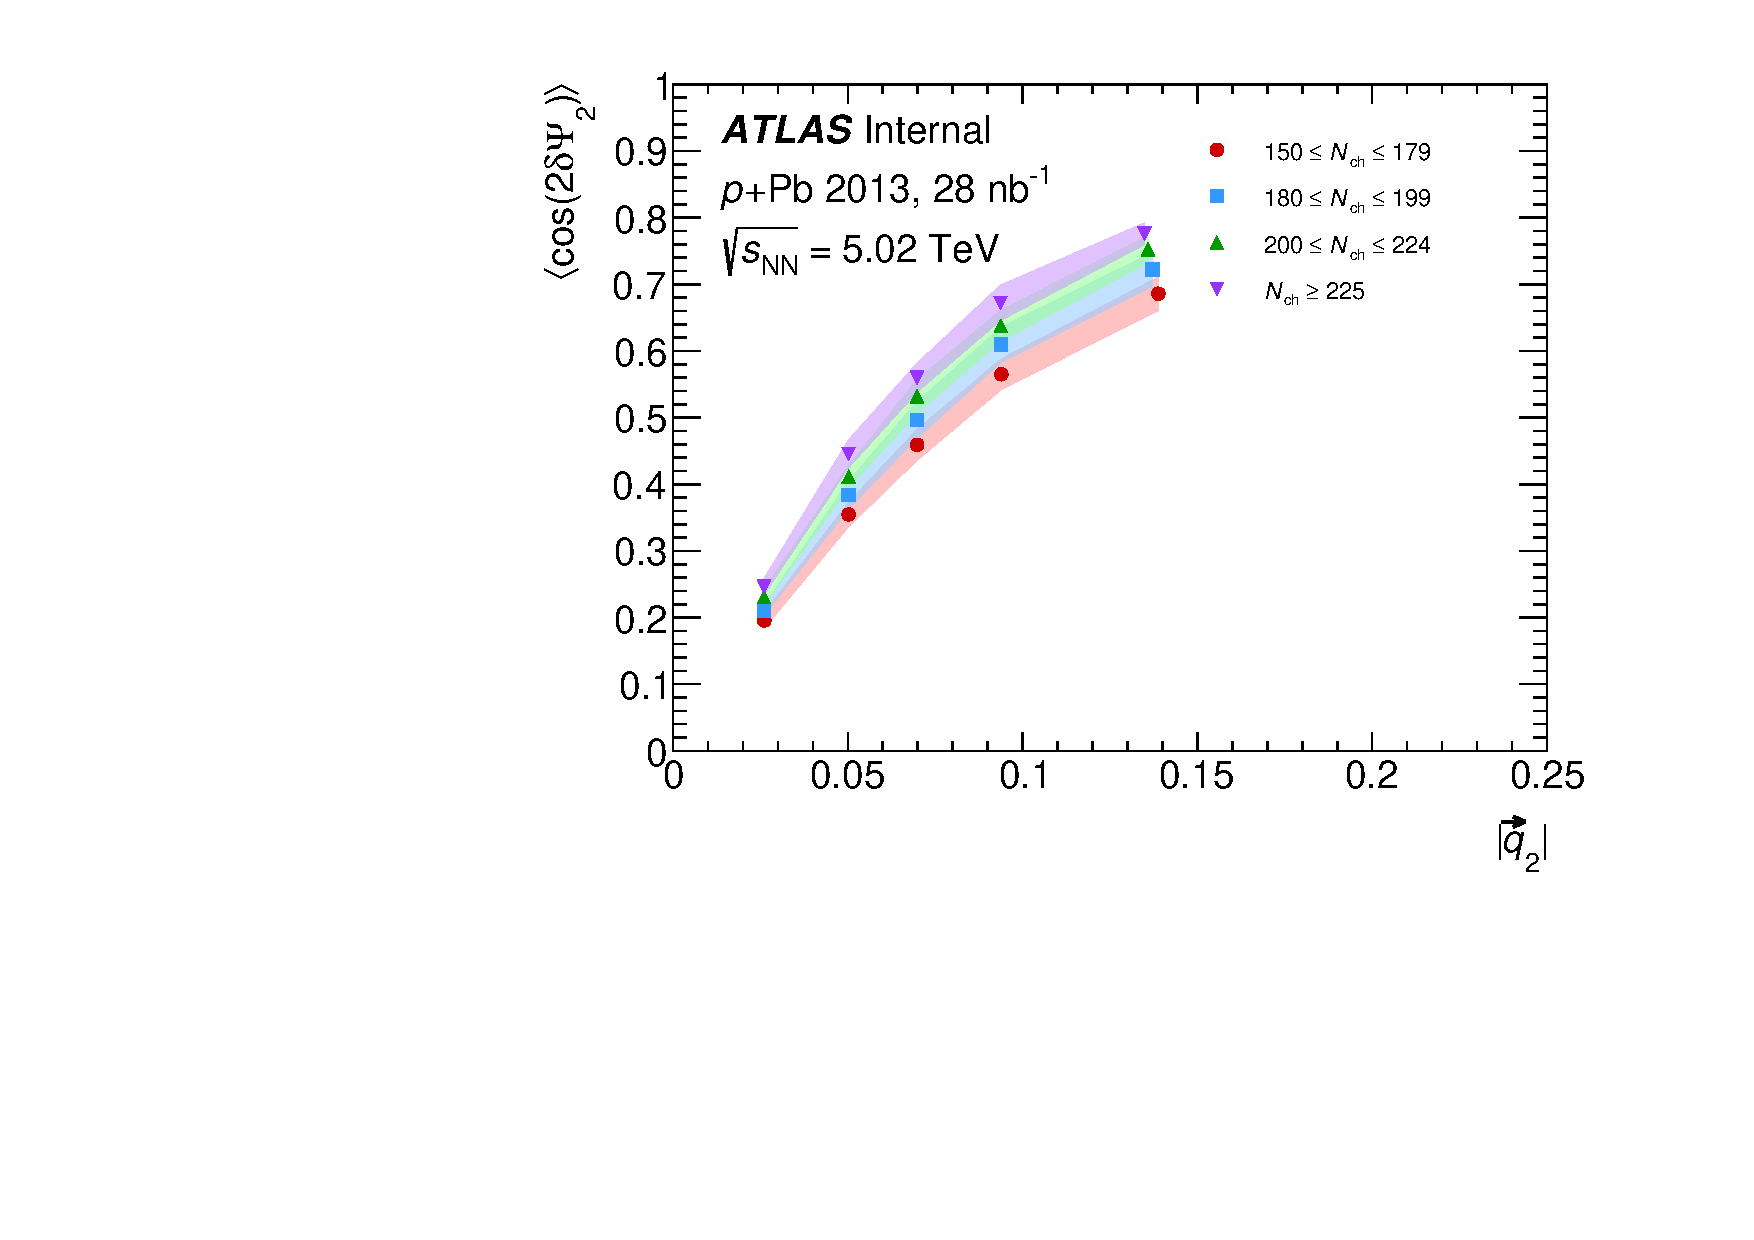
\includegraphics{epRes.pdf}\\
\caption{The event plane resolution as a function of the magnitude of the flow vector $|\qt|$ calculated using calorimeter cells with $\eta < -2.5$. Four different intervals of reconstructed track multiplicity \Nch used in the analysis are shown. The systematic uncertainties are shown in the bands, and statistical uncertainties are too small to be visible.}
\label{fig:ep_res}
\end{figure}


\section{Correlation function}

\subsection{Coulomb correction}
The residual strong force between charged pions is subdominant to the Coulomb effect and can be neglected \cite{Lednicky:2005tb} in final-state effects.
In heavy ion collisions the Bohr radius of a pair of pions ($a_{\pi} = 387.5 \textrm{ fm}$) is significantly larger than the source size, which is on the order of a few fermi.
The nonrelativistic limit is appropriate since in the region of interest the pions have low relative momentum.
In the limit where the pions come from a point source, their outgoing wavefunction squared is given by the Gamow factor

\begin{equation} \frac{\left| \psi (q, r=0) \right|^2}{\left| \psi (q, r\rightarrow\infty) \right|^2} = G(\qinv) \equiv \frac{4\pi}{a \qinv}\frac{1}{e^{\frac{4\pi}{a \qinv}} - 1} \end{equation}

where $a$ is the Bohr radius.
(The literature contains various conventions for the factors of 2.
Here the Bohr radius contains the reduced mass and this definition of $q$ has no factor of $1/2$.)
For opposite-charged pairs, the correction can be applied by taking $a \to -a$, as this effectively flips the sign of the coupling constant $\alpha_{EM}$.

For a source that is extended in space, a correction to this expression is required.
For a spherical Gaussian source of effective size \Reff, the formula for a more precise correction factor $K(\qinv)$ is calculated in \Ref{\cite{Maj:2009ue}} in terms of a generalized hypergeometric function ${}_2 F_2$.
\begin{equation} K(\qinv) = G(\qinv) \left[ 1 + \frac{8\Reff}{\sqrt{\pi}a} {}_2 F_2 \left( \frac{1}{2}, 1; \frac{3}{2}, \frac{3}{2}; -\Reff^2 \qinv^2 \right) \right] \end{equation}
The analytic gradient of the correlation function parameterization is used in the fitting algorithm, so the derivative with respect to \Reff is also required:
\begin{equation}
  \frac{\partial K(\qinv)}{\partial \Reff} = G(\qinv) \frac{8}{\sqrt{\pi}a} {}_1 F_1 \left( 1; \frac{3}{2}; -\Reff^2 \qinv^2 \right) \; .
\end{equation}
The effective size \Reff described here cannot be connected \emph{a priori} to the HBT radii without additional model-dependent assumptions.
It is taken to be proportional to \Rinv with the constant of proportionality adjusted as a systematic variation.

Implementations of ${}_2F_2 (a_1, a_2; b_1, b_2; z)$ are not generally available.
%% Series approximations for this function are produced here at small and large negative $z$ (used with a cutoff around $z \approx -18$), respectively.
A series expansion around small $z$ follows direction from the definition.
\begin{equation} {}_2F_2 \left( \frac{1}{2}, 1; \frac{3}{2}, \frac{3}{2}; z \right) = \sum_{n=0}^{\infty} \frac{z^n}{(2n+1) \left(\frac{3}{2}\right)_n} \end{equation}
The Pochhammer symbol $(a)_n$ is used to denote the rising factorial $(a)_n \equiv a(a+1)...(a+n-1) = \frac{\Gamma(a+n)}{\Gamma(a)}$.
An asymptotic expansion around $z \to - \infty$ can be derived.
\begin{equation} {}_2F_2 \left( \frac{1}{2}, 1; \frac{3}{2}, \frac{3}{2}; z \right) \approx \frac{\pi^{3/2}}{4\sqrt{-z}} - \sum_{n=1}^{n < |z| + 3/2} \frac{(2n-3)!!}{(2n-1) 2^n |z|^n}  \end{equation}
This expression is a formally divergent asymptotic series for large negative $z$, so the cutoff is chosen after the smallest term.
In practice it agrees to within several digits of precision relatively quickly.

Corresponding expressions for the confluent hypergeometric function appearing in the derivative are given by:
\begin{equation}
 {}_1F_1 \left( 1;\frac{3}{2}; z \right) = \sum_{n=0}^{\infty} \frac{z^n}{\left(\frac{3}{2}\right)_n} 
\end{equation}
\begin{equation}
  {}_1F_1 \left( 1; \frac{3}{2}; z \right) \approx \sum_{n=1}^{n < |z| + 3/2} \frac{(2n-3)!!}{2^n |z|^n} \; \textrm{for } z \rightarrow -\infty
\end{equation}

To apply the Coulomb correction in 3D out-side-long coordinates, the average \kt in each bin is used to contract compute \qinv from $\mathbf{q}$.
The following expression takes advantage of working in the \ac{LCMF} so that $k_L = 0$.
\begin{equation}
\qinv^2 = |\mathbf{q}|^2 - \Gamma^2 + \sqrt{\Gamma^4 - 4 |\mathbf{k}_\mathrm{T}|^2 \qout^2} \label{eqn:q3_to_qinv}
\end{equation}
where
\begin{equation}
\Gamma^2 = 2 m_{\pi}^2 + 2 |\mathbf{k}_\mathrm{T}|^2 + \frac{1}{2}|\mathbf{q}|^2 \; .
\end{equation}


\section{Fragmentation background}
\section{Fit procedure}
\section{Systematic uncertainties}
